
% Copyright (c) Gustavo T. Pfeiffer 2025.
\documentclass{beamer}
\usetheme{Madrid}
\usefonttheme{serif}
\usepackage{tikz}
\usetikzlibrary{arrows.meta}
\usepackage{amsmath}
\usepackage{amssymb}
\usepackage{txfonts}
\usepackage[utf8]{inputenc}
\hyphenpenalty = 100000000
\sloppypar

\title{Atrasos em filtros de Kalman}
\author{Gustavo T. Pfeiffer}
\date{19/8/2025}

%\def\Put(#1,#2)#3{\leavevmode\makebox(0,0){\put(#1,#2){#3}}}
%\usepackage[overlay, absolute]{textpos}

\begin{document}

\maketitle

\begin{frame}\frametitle{Agenda}
\begin{itemize}
	\item 1. Filtro de Kalman: O que é, para que serve
	\item 2. Modelo matemático
	\item 3. Problema dos atrasos
	\item 4. Solução
\end{itemize}
\end{frame}

\begin{frame}\frametitle{O que é um filtro de Kalman}
\begin{itemize}
	\item Sistema $X(t)$ evolui estocasticamente no tempo

\vfill
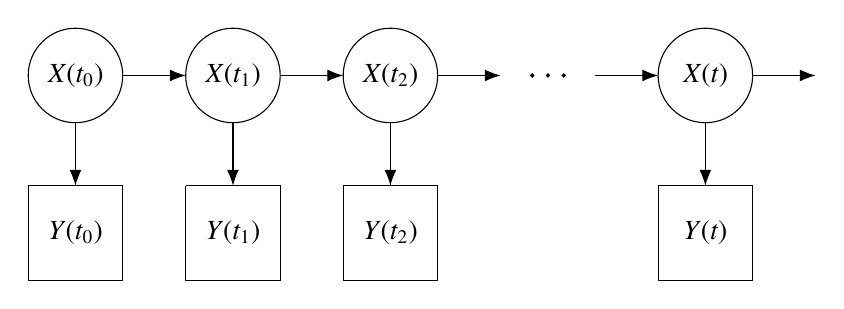
\begin{tikzpicture}
\draw
  (0,0) circle [radius=0.6cm] node {$X(t_0)$}
  (2,0) circle [radius=0.6cm] node {$X(t_1)$}
  (4,0) circle [radius=0.6cm] node {$X(t_2)$}
  (8,0) circle [radius=0.6cm] node {$X(t)$};
\filldraw
  (5.8,0) circle [radius=0.2mm]
  (6,0) circle [radius=0.2mm]
  (6.2,0) circle [radius=0.2mm];
\draw[-{Latex[length=2mm]}] (0.6,0) -- (1.4,0);
\draw[-{Latex[length=2mm]}] (2.6,0) -- (3.4,0);
\draw[-{Latex[length=2mm]}] (4.6,0) -- (5.4,0);
\draw[-{Latex[length=2mm]}] (6.6,0) -- (7.4,0);
\draw[-{Latex[length=2mm]}] (8.6,0) -- (9.4,0);
\draw[-{Latex[length=2mm]}] (0,-0.6) -- (0,-1.4);
\draw[-{Latex[length=2mm]}] (2,-0.6) -- (2,-1.4);
\draw[-{Latex[length=2mm]}] (4,-0.6) -- (4,-1.4);
\draw[-{Latex[length=2mm]}] (8,-0.6) -- (8,-1.4);
\draw (-0.6,-1.4) -- (-0.6,-2.6) -- (0.6,-2.6) -- (0.6,-1.4) -- (-0.6,-1.4) (0,-2) node {$Y(t_0)$};
\draw (1.4,-1.4) -- (1.4,-2.6) -- (2.6,-2.6) -- (2.6,-1.4) -- (1.4,-1.4) (2,-2) node {$Y(t_1)$};
\draw (3.4,-1.4) -- (3.4,-2.6) -- (4.6,-2.6) -- (4.6,-1.4) -- (3.4,-1.4) (4,-2) node {$Y(t_2)$};
\draw (7.4,-1.4) -- (7.4,-2.6) -- (8.6,-2.6) -- (8.6,-1.4) -- (7.4,-1.4) (8,-2) node {$Y(t)$};
\end{tikzpicture}
\vfill

	\item Medidas $Y(t)$ com erros aleatórios
	\item Objetivo: Estimar $X(t)$ dadas todas as medições $Y(0)$, ..., $Y(t)$ em tempo real
\end{itemize}
\end{frame}

\begin{frame}\frametitle{Exemplo}
\textbf{Movimento browniano}

\vfill
\text{ }\text{ }\text{ }\text{ }\text{ }\text{ }\text{ }\text{ }\text{ }\text{ }
\text{ }\text{ }\text{ }\text{ }\text{ }\text{ }\text{ }\text{ }
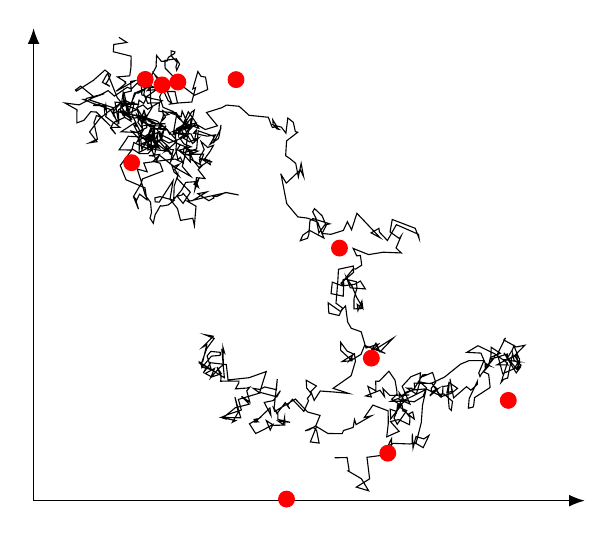
\begin{tikzpicture}
\draw[-{Latex[length=2mm]}] (0,0.5) -- (7,0.5);
\draw[-{Latex[length=2mm]}] (0,0.5) -- (0,6.5);
\draw 
(3.8219,1.0444) -- (3.9816,1.0480) -- (4.0074,0.8831) -- (3.9932,0.8783) -- (4.1636,0.7785) -- (4.2551,0.6255) -- (4.0990,0.6721) -- (4.2677,0.7772) -- (4.2339,1.0508) -- (4.4336,1.0774) -- (4.5433,1.0974) -- (4.5467,1.2875) -- (4.5227,1.2430) -- (4.5011,1.1921) -- (4.5705,1.2277) -- (4.7777,1.2199) -- (4.8483,1.2320) -- (4.9482,1.1733) -- (5.0213,1.3286) -- (4.9561,1.2842) -- (4.8572,1.3158) -- (4.8190,1.1692) -- (4.8106,1.3520) -- (4.8067,1.2340) -- (4.8562,1.2249) -- (4.9240,1.4940) -- (4.9395,1.7137) -- (4.9896,1.9337) -- (4.9058,2.0078) -- (4.9925,1.9913) -- (5.0614,1.9866) -- (5.1634,1.8293) -- (5.1406,1.8443) -- (5.1680,1.8173) -- (5.3068,1.8651) -- (5.3845,1.9264) -- (5.2760,2.0016) -- (5.2491,1.8700) -- (5.3144,1.8885) -- (5.2884,2.0474) -- (5.3341,1.8056) -- (5.4980,1.9479) -- (5.5539,1.9029) -- (5.6347,1.9767) -- (5.6362,2.0161) -- (5.5320,1.7967) -- (5.5218,1.6743) -- (5.5805,1.6884) -- (5.5883,1.7028) -- (5.6004,1.8084) -- (5.7984,1.9379) -- (5.7789,2.1064) -- (5.7134,2.1368) -- (5.7740,2.2042) -- (5.8020,2.3189) -- (5.9277,2.3718) -- (5.8123,2.4478) -- (5.8066,2.2981) -- (6.0177,2.3625) -- (6.0106,2.3013) -- (6.0784,2.4113) -- (6.1006,2.4673) -- (6.1726,2.2875) -- (6.1654,2.2571) -- (6.1855,2.1984) -- (6.1299,2.1226) -- (5.9727,2.3778) -- (6.1297,2.1764) -- (6.1554,2.2182) -- (6.1347,2.3500) -- (5.9976,2.2851) -- (5.8858,2.2260) -- (6.0240,2.2237) -- (5.9801,2.2916) -- (6.1742,2.2610) -- (6.1590,2.2602) -- (6.1094,2.3421) -- (6.2393,2.4737) -- (6.1304,2.4525) -- (5.9726,2.5407) -- (5.9933,2.5674) -- (5.8907,2.3613) -- (5.9578,2.1122) -- (6.1050,2.1768) -- (6.1652,2.2784) -- (6.1496,2.1744) -- (6.1330,2.1618) -- (6.1901,2.2217) -- (6.1011,2.2875) -- (6.0839,2.3690) -- (6.0204,2.0572) -- (5.9715,2.0419) -- (5.9375,2.0024) -- (6.0166,2.2491) -- (5.8581,2.3644) -- (5.6434,2.4677) -- (5.5021,2.3836) -- (5.6815,2.3742) -- (5.7353,2.2464) -- (5.7928,2.2128) -- (5.7358,2.2321) -- (5.7358,2.1913) -- (5.8609,2.3277) -- (5.6850,2.1067) -- (5.6692,2.0761) -- (5.6537,2.1208) -- (5.7193,2.2783) -- (5.5305,2.2787) -- (5.4221,2.2335) -- (5.2209,2.0708) -- (5.0486,1.9887) -- (4.8342,1.9929) -- (4.8404,1.9186) -- (4.6676,1.8325) -- (4.7728,1.8434) -- (4.5232,1.8364) -- (4.4364,1.9250) -- (4.4559,1.8231) -- (4.3997,1.9019) -- (4.2180,1.8302) -- (4.2890,1.8170) -- (4.2462,1.9505) -- (4.3477,1.8956) -- (4.3452,2.0183) -- (4.3878,2.0158) -- (4.5125,2.1437) -- (4.5900,2.0307) -- (4.6123,1.9051) -- (4.6153,1.8513) -- (4.5485,1.7884) -- (4.6671,1.7072) -- (4.5357,1.5392) -- (4.5291,1.6617) -- (4.6069,1.6339) -- (4.7157,1.8727) -- (4.7979,1.9014) -- (4.8344,1.9221) -- (4.9407,2.0974) -- (4.9802,2.0999) -- (4.9232,2.0684) -- (5.0672,2.1280) -- (5.1066,2.0023) -- (5.0486,1.9235) -- (5.0561,1.8820) -- (5.1374,1.9226) -- (5.0360,1.8433) -- (5.0377,1.8341) -- (5.1293,1.9135) -- (5.0831,1.9576) -- (5.1731,1.8238) -- (5.1960,1.8711) -- (5.1982,1.9489) -- (5.2646,1.9607) -- (5.2764,1.9669) -- (5.2630,1.8454) -- (5.2782,1.6736) -- (5.3053,1.6463) -- (5.3200,1.7614) -- (5.2104,1.8558) -- (5.1286,1.8495) -- (4.9827,1.9203) -- (4.8131,1.9040) -- (4.8057,1.9274) -- (4.7412,1.9299) -- (4.8610,1.8552) -- (4.8999,1.9842) -- (4.9132,2.1229) -- (4.7923,2.0740) -- (4.6808,1.9524) -- (4.7799,1.7268) -- (4.6562,1.7812) -- (4.8328,1.7549) -- (4.9461,1.8241) -- (4.9813,1.9116) -- (4.7065,1.7750) -- (4.6437,1.8682) -- (4.6538,1.8069) -- (4.5407,1.7626) -- (4.7127,1.7622) -- (4.6304,1.6936) -- (4.7386,1.6439) -- (4.6181,1.4703) -- (4.5778,1.5507) -- (4.6106,1.6231) -- (4.6227,1.7174) -- (4.6790,1.7177) -- (4.6953,1.6303) -- (4.6870,1.6538) -- (4.8353,1.5356) -- (4.8150,1.6266) -- (4.7514,1.5935) -- (4.7797,1.5608) -- (4.7756,1.4640) -- (4.6354,1.5303) -- (4.5334,1.5040) -- (4.6421,1.3805) -- (4.4849,1.3105) -- (4.5045,1.4787) -- (4.5029,1.6403) -- (4.3098,1.7139) -- (4.2001,1.5566) -- (4.2889,1.5770) -- (4.0960,1.4658) -- (4.0754,1.5296) -- (4.0585,1.4297) -- (3.9375,1.3916) -- (3.9176,1.3507) -- (3.7375,1.3534) -- (3.5935,1.4411) -- (3.5147,1.2461) -- (3.6262,1.2315) -- (3.5941,1.3935) -- (3.5505,1.4315) -- (3.4484,1.3868) -- (3.5046,1.4013) -- (3.5844,1.4512) -- (3.6379,1.5824) -- (3.4797,1.6266) -- (3.3250,1.7907) -- (3.0634,1.6334) -- (3.0496,1.6710) -- (3.1019,1.6059) -- (3.1022,1.5321) -- (3.2576,1.4955) -- (3.1051,1.5108) -- (3.1705,1.4680) -- (3.1882,1.5576) -- (3.1919,1.4598) -- (3.0508,1.4568) -- (2.9560,1.5164) -- (3.0055,1.3969) -- (3.0390,1.4668) -- (2.9099,1.3956) -- (2.8205,1.3532) -- (2.7411,1.4762) -- (2.8562,1.5417) -- (2.8048,1.5323) -- (2.8524,1.5011) -- (2.8143,1.4981) -- (3.0016,1.6763) -- (3.0140,1.5836) -- (2.9295,1.7476) -- (3.0451,1.7716) -- (3.1343,1.8972) -- (3.0899,1.8182) -- (2.8724,1.8771) -- (2.9547,2.1397) -- (2.7367,2.0616) -- (2.4699,2.0334) -- (2.4478,2.2283) -- (2.2440,2.2522) -- (2.2439,2.2433) -- (2.1548,2.1212) -- (2.1989,2.1955) -- (2.1066,2.2485) -- (2.1477,2.2620) -- (2.1990,2.4792) -- (2.1445,2.4484) -- (2.2817,2.5884) -- (2.1750,2.6081) -- (2.2933,2.5601) -- (2.1983,2.4312) -- (2.1288,2.2357) -- (2.1371,2.1903) -- (2.2590,2.3356) -- (2.3694,2.3451) -- (2.3719,2.3837) -- (2.2498,2.3956) -- (2.2034,2.3374) -- (2.2566,2.1644) -- (2.1453,2.1947) -- (2.1109,2.2569) -- (2.4229,2.0612) -- (2.3912,2.4127) -- (2.4248,2.3781) -- (2.4042,2.4501) -- (2.4099,2.2266) -- (2.3553,2.1826) -- (2.2503,2.0631) -- (2.2974,2.1790) -- (2.1806,2.1154) -- (2.2634,2.0708) -- (2.3846,2.1118) -- (2.3298,2.1956) -- (2.3812,2.0764) -- (2.3767,2.0172) -- (2.6078,2.0182) -- (2.6063,1.9953) -- (2.5642,1.9194) -- (2.7111,1.9304) -- (2.7455,1.9414) -- (2.7074,1.8931) -- (2.7466,1.7504) -- (2.6416,1.8251) -- (2.7402,1.7259) -- (2.5617,1.6800) -- (2.4022,1.5496) -- (2.4519,1.5341) -- (2.4290,1.5464) -- (2.5682,1.5182) -- (2.5253,1.4963) -- (2.6005,1.6244) -- (2.5571,1.8163) -- (2.6307,1.5527) -- (2.3822,1.5574) -- (2.4693,1.5949) -- (2.6390,1.6520) -- (2.6009,1.7858) -- (2.8727,1.8670) -- (2.7903,1.9264) -- (2.8729,1.9124) -- (2.9341,1.9444) -- (3.0834,1.9095) -- (3.0947,2.0445) -- (3.0546,1.6734) -- (3.0913,1.6063) -- (3.1959,1.7449) -- (3.2517,1.6658) -- (3.2254,1.7140) -- (3.2869,1.7870) -- (3.4326,1.6339) -- (3.4916,1.7680) -- (3.4770,1.7987) -- (3.5268,1.8591) -- (3.4687,1.9310) -- (3.4622,2.0296) -- (3.5915,1.9570) -- (3.5218,1.8857) -- (3.5636,1.7739) -- (3.6404,1.8926) -- (3.8189,1.8797) -- (4.0029,1.8615) -- (3.8043,1.9267) -- (4.0332,2.0870) -- (4.0877,2.2718) -- (4.0742,2.3652) -- (3.9191,2.2674) -- (4.0451,2.2773) -- (4.0457,2.3048) -- (4.0082,2.2752) -- (4.0631,2.3633) -- (3.9817,2.3997) -- (3.9009,2.5099) -- (3.8999,2.4096) -- (4.0362,2.2841) -- (4.1577,2.3578) -- (4.2044,2.4726) -- (4.3218,2.4246) -- (4.4669,2.3700) -- (4.3493,2.4272) -- (4.5673,2.5653) -- (4.3993,2.3889) -- (4.3477,2.5006) -- (4.2618,2.3671) -- (4.3784,2.4876) -- (4.2219,2.4388) -- (4.1602,2.6450) -- (4.0342,2.6891) -- (3.9886,2.7696) -- (3.9615,2.9739) -- (3.8977,2.9029) -- (3.7406,3.0128) -- (3.7499,2.8819) -- (3.8795,2.8512) -- (3.9242,2.9459) -- (3.8407,3.0079) -- (3.8634,3.2823) -- (3.8722,3.4387) -- (4.0615,3.4797) -- (4.0629,3.3980) -- (3.9035,3.2626) -- (3.9265,3.2317) -- (3.9311,3.3156) -- (3.9393,3.2572) -- (3.9321,3.0970) -- (3.7778,3.1296) -- (3.7938,3.2749) -- (3.9235,3.2272) -- (4.0838,3.2496) -- (4.1504,3.2896) -- (4.2128,3.1890) -- (4.0217,3.2031) -- (3.9752,3.3321) -- (4.0496,3.2105) -- (4.0341,3.2505) -- (4.1028,3.0820) -- (4.1805,2.9503) -- (4.1696,3.0346) -- (4.1194,2.9146) -- (4.1104,2.9930) -- (4.1761,2.9385) -- (4.0689,2.9361) -- (4.0700,3.0713) -- (4.1074,3.2018) -- (4.0991,3.2801) -- (3.9539,3.3158) -- (4.0594,3.4444) -- (4.0928,3.4422) -- (4.1674,3.4915) -- (4.1507,3.6142) -- (4.1042,3.6089) -- (4.0584,3.7036) -- (4.2547,3.6251) -- (4.4404,3.6553) -- (4.6685,3.6460) -- (4.6035,3.7101) -- (4.6678,3.8613) -- (4.6445,3.8296) -- (4.5273,3.9130) -- (4.5549,4.0709) -- (4.8468,3.9591) -- (4.8956,3.8312) -- (4.8883,3.8826) -- (4.6077,4.0050) -- (4.4936,3.8041) -- (4.3917,3.9112) -- (4.3861,3.9580) -- (4.2869,3.9015) -- (4.4002,3.8400) -- (4.1063,4.1495) -- (4.0387,3.9408) -- (3.9853,4.0426) -- (3.9340,3.9321) -- (3.7745,3.8820) -- (3.7687,3.8828) -- (3.6632,3.8939) -- (3.7156,3.9934) -- (3.6652,4.1168) -- (3.5680,4.2091) -- (3.5445,4.1682) -- (3.5887,4.0811) -- (3.6230,3.8999) -- (3.6965,4.0006) -- (3.7611,4.0156) -- (3.5473,4.0827) -- (3.5093,4.0519) -- (3.4963,3.8830) -- (3.4788,3.8326) -- (3.3877,3.8009) -- (3.4180,3.8709) -- (3.5048,3.9324) -- (3.6869,3.8353) -- (3.6069,4.0382) -- (3.4799,4.0881) -- (3.3562,4.1039) -- (3.2148,4.2729) -- (3.1437,4.6384) -- (3.1372,4.6527) -- (3.2087,4.5340) -- (3.2208,4.5426) -- (3.3883,4.7016) -- (3.4290,4.6162) -- (3.3981,4.7827) -- (3.3629,4.6119) -- (3.3289,4.7837) -- (3.2585,4.8420) -- (3.2012,4.8807) -- (3.2133,5.0697) -- (3.3546,5.1788) -- (3.3244,5.1871) -- (3.2988,5.3049) -- (3.2290,5.3599) -- (3.2044,5.1669) -- (3.1477,5.2435) -- (3.0496,5.2682) -- (3.1172,5.2163) -- (3.0897,5.2215) -- (3.0429,5.2748) -- (3.0380,5.3356) -- (3.0917,5.2490) -- (3.0343,5.2398) -- (3.0219,5.2599) -- (2.9821,5.3689) -- (2.7364,5.3943) -- (2.6107,5.5084) -- (2.4497,5.5240) -- (2.3907,5.4910) -- (2.1961,5.4293) -- (2.3349,5.2607) -- (2.1814,5.2135) -- (2.0781,5.2730) -- (1.9322,5.2224) -- (1.9074,5.2274) -- (1.9775,5.3310) -- (2.0055,5.3560) -- (1.9508,5.1006) -- (1.9404,5.0128) -- (2.0286,4.8202) -- (2.1006,4.7315) -- (2.2351,4.8217) -- (2.2447,4.7687) -- (2.1082,4.8559) -- (2.1665,4.9595) -- (2.1269,5.0615) -- (2.2115,4.9852) -- (2.2847,5.0121) -- (2.2394,4.9330) -- (2.1676,4.8338) -- (2.2700,4.7996) -- (2.1778,4.8401) -- (2.1057,4.8339) -- (2.1157,4.7840) -- (2.1599,4.9008) -- (1.9346,4.8967) -- (1.9687,4.8871) -- (2.0877,4.9400) -- (1.9804,4.9564) -- (1.9898,4.8032) -- (1.8545,4.9547) -- (1.8971,4.9166) -- (2.0712,4.9663) -- (2.0906,5.1971) -- (2.2876,5.1278) -- (2.2926,5.0552) -- (2.3475,5.1675) -- (2.3779,5.2232) -- (2.3798,5.2729) -- (2.3610,5.1521) -- (2.3477,5.0983) -- (2.2400,5.0245) -- (2.3104,5.1462) -- (2.2044,5.1292) -- (2.0303,5.1667) -- (2.0696,5.2105) -- (2.0435,5.0689) -- (2.0000,5.1583) -- (1.8992,5.1648) -- (1.7905,5.1752) -- (1.8162,5.0406) -- (1.9484,4.9859) -- (1.8886,4.7450) -- (1.9968,4.6174) -- (1.7577,4.7537) -- (1.7849,4.6713) -- (1.8464,4.6223) -- (1.7915,4.7090) -- (1.8488,4.7718) -- (1.7819,4.7442) -- (1.5982,4.8874) -- (1.5165,4.8101) -- (1.6057,4.7862) -- (1.6429,4.6860) -- (1.3852,4.5874) -- (1.3603,4.5162) -- (1.2679,4.3620) -- (1.3322,4.2029) -- (1.2915,4.3380) -- (1.3087,4.3169) -- (1.3468,4.3930) -- (1.4378,4.3219) -- (1.4151,4.4725) -- (1.1739,4.5755) -- (1.1004,4.7574) -- (1.2470,4.9530) -- (1.0859,4.9557) -- (1.1715,5.0793) -- (1.2017,5.1278) -- (1.3777,5.1180) -- (1.5176,4.9801) -- (1.4516,4.9534) -- (1.4419,5.0235) -- (1.4438,5.0145) -- (1.5357,5.2335) -- (1.5364,5.0988) -- (1.5838,4.9995) -- (1.4933,4.9767) -- (1.4509,5.0096) -- (1.4754,5.1690) -- (1.5481,5.2820) -- (1.6760,5.2860) -- (1.5616,5.2879) -- (1.3907,5.3723) -- (1.4778,5.3184) -- (1.3641,5.4026) -- (1.3117,5.4895) -- (1.3901,5.5248) -- (1.4479,5.4707) -- (1.6326,5.5792) -- (1.4935,5.6091) -- (1.3748,5.6537) -- (1.3641,5.8766) -- (1.4756,5.8032) -- (1.4171,5.7404) -- (1.4461,5.7815) -- (1.3473,5.7766) -- (1.4284,5.7386) -- (1.2996,5.6821) -- (1.2411,5.5506) -- (1.2836,5.5612) -- (1.1068,5.5141) -- (1.1736,5.4138) -- (1.1381,5.3911) -- (1.1089,5.4509) -- (1.2774,5.3949) -- (1.3841,5.3587) -- (1.3879,5.3162) -- (1.3509,5.3499) -- (1.3119,5.4006) -- (1.3304,5.3367) -- (1.4232,5.3825) -- (1.3788,5.3197) -- (1.4924,5.2395) -- (1.5236,5.1070) -- (1.5331,5.2202) -- (1.6990,5.2142) -- (1.7333,5.1463) -- (1.6983,5.2082) -- (1.7979,5.0978) -- (1.8095,5.1772) -- (1.8158,5.2234) -- (1.9325,5.2903) -- (2.0970,5.2308) -- (2.0546,5.3120) -- (1.9649,5.4391) -- (1.8433,5.1422) -- (1.8434,5.2081) -- (1.9693,5.2606) -- (1.8866,5.4480) -- (1.8745,5.3760) -- (1.7072,5.4343) -- (1.8100,5.4281) -- (1.8539,5.3646) -- (1.7688,5.4445) -- (1.6441,5.4950) -- (1.6003,5.6286) -- (1.6599,5.7482) -- (1.6045,5.8024) -- (1.7099,5.5784) -- (1.7643,5.5410) -- (1.7757,5.5391) -- (1.7579,5.5418) -- (1.6610,5.7890) -- (1.5380,5.9118) -- (1.6700,5.6957) -- (1.7953,5.6967) -- (1.8278,5.5493) -- (1.7156,5.5341) -- (1.8310,5.5501) -- (2.0095,5.5626) -- (2.0568,5.7450) -- (2.0223,5.7294) -- (2.0865,5.9501) -- (2.1263,5.8883) -- (2.1837,5.8796) -- (2.2111,5.7214) -- (2.0442,5.6492) -- (1.9137,5.7474) -- (1.6701,5.9939) -- (1.6680,6.0917) -- (1.8126,6.1117) -- (1.8546,6.0445) -- (1.8180,5.9664) -- (1.8076,6.0074) -- (1.8244,6.0664) -- (1.7473,6.1502) -- (1.7473,6.2129) -- (1.7953,6.1994) -- (1.7901,6.1794) -- (1.7113,6.1302) -- (1.6960,6.0839) -- (1.6229,6.0786) -- (1.5621,6.1543) -- (1.5566,6.0415) -- (1.5580,6.0160) -- (1.4958,5.8942) -- (1.3791,5.8302) -- (1.5318,5.7480) -- (1.4258,5.7435) -- (1.4114,5.7192) -- (1.3284,5.6750) -- (1.2826,5.6792) -- (1.2096,5.4330) -- (1.1963,5.5142) -- (1.1487,5.3636) -- (1.0163,5.3035) -- (0.9768,5.2334) -- (1.0429,5.1551) -- (0.9805,5.2407) -- (1.0955,5.2417) -- (0.9153,5.3775) -- (0.9310,5.4276) -- (1.1027,5.5460) -- (1.0212,5.4537) -- (1.0153,5.3803) -- (1.0109,5.4905) -- (0.7036,5.5917) -- (0.8535,5.5390) -- (0.8250,5.5285) -- (0.7554,5.5195) -- (0.8984,5.5143) -- (0.9013,5.4513) -- (0.9170,5.5249) -- (0.9274,5.4201) -- (0.8426,5.3568) -- (0.7109,5.1830) -- (0.8045,5.0598) -- (0.7088,5.0441) -- (0.8110,5.0907) -- (0.7868,5.2057) -- (0.7670,5.2997) -- (0.7980,5.3891) -- (0.8572,5.3729) -- (0.9731,5.2612) -- (0.7959,5.4357) -- (0.7502,5.4380) -- (0.7277,5.4411) -- (0.6392,5.3300) -- (0.5493,5.2978) -- (0.5510,5.4642) -- (0.3980,5.5503) -- (0.5788,5.5268) -- (0.7696,5.6253) -- (0.5972,5.7644) -- (0.5318,5.7158) -- (0.5426,5.7004) -- (0.7585,5.8371) -- (0.9067,5.9688) -- (0.9782,5.9094) -- (0.9398,5.8257) -- (0.9163,5.7977) -- (0.9691,5.7617) -- (0.8745,5.8117) -- (0.9266,5.9078) -- (0.9414,5.9217) -- (0.9835,5.8172) -- (1.0628,5.6181) -- (1.1485,5.5146) -- (1.1796,5.5357) -- (1.0765,5.4621) -- (1.0836,5.2809) -- (1.0339,5.5621) -- (1.2738,5.5364) -- (1.2461,5.4100) -- (1.3657,5.1612) -- (1.2449,5.1927) -- (1.3422,5.0928) -- (1.3411,4.9242) -- (1.5345,5.0194) -- (1.5064,4.9422) -- (1.5596,4.8160) -- (1.6016,4.8976) -- (1.4660,4.8802) -- (1.5359,4.8760) -- (1.5747,5.1145) -- (1.4171,5.0341) -- (1.4849,5.2230) -- (1.6556,5.2246) -- (1.6821,5.2622) -- (1.6175,5.1464) -- (1.7000,5.1082) -- (1.8621,5.0159) -- (1.8396,4.9846) -- (1.7416,4.8089) -- (1.7588,4.9021) -- (1.7777,4.9589) -- (1.7412,4.9581) -- (1.6936,5.0150) -- (1.6056,5.0877) -- (1.5938,5.0548) -- (1.4047,5.0974) -- (1.6028,5.1881) -- (1.6280,5.0937) -- (1.6543,5.2049) -- (1.6947,5.2099) -- (1.5674,5.3205) -- (1.3897,5.3727) -- (1.3778,5.2807) -- (1.5062,5.4952) -- (1.4863,5.5504) -- (1.4826,5.7439) -- (1.4320,5.8346) -- (1.4004,5.6624) -- (1.4505,5.5453) -- (1.4867,5.5510) -- (1.5987,5.5520) -- (1.5905,5.4480) -- (1.6383,5.4384) -- (1.6758,5.3713) -- (1.6403,5.3327) -- (1.6471,5.4071) -- (1.6386,5.4545) -- (1.7158,5.4041) -- (1.6484,5.3892) -- (1.5840,5.2227) -- (1.6370,5.2575) -- (1.4157,5.2644) -- (1.5239,5.2877) -- (1.4543,5.3259) -- (1.4016,5.4540) -- (1.3626,5.3358) -- (1.5732,5.2115) -- (1.6136,5.0969) -- (1.7196,5.0418) -- (1.7299,5.0461) -- (1.9508,5.1307) -- (1.8080,5.1691) -- (1.7722,5.1516) -- (1.8133,5.3835) -- (1.9749,5.2345) -- (1.8938,5.2499) -- (1.9087,5.2532) -- (1.7691,5.1885) -- (1.9288,5.2142) -- (1.9510,5.1430) -- (2.0195,5.0354) -- (2.0962,5.1068) -- (1.9807,5.0576) -- (1.9089,5.1003) -- (1.9667,5.2226) -- (2.0172,5.2863) -- (2.0602,5.2951) -- (1.9851,5.2137) -- (2.0410,5.4598) -- (2.0059,5.4341) -- (1.9897,5.4047) -- (1.8718,5.2133) -- (1.9174,5.1408) -- (1.8563,5.1073) -- (1.9073,5.0312) -- (2.0003,4.9940) -- (1.8410,4.9491) -- (1.8972,4.9049) -- (1.9151,4.9953) -- (2.0288,4.9198) -- (1.9471,4.9572) -- (2.0044,4.9408) -- (1.9872,4.8401) -- (2.1407,4.7550) -- (2.0903,4.7026) -- (2.1780,4.5908) -- (2.0687,4.6020) -- (2.0487,4.4499) -- (2.0975,4.5850) -- (2.0373,4.5180) -- (2.0937,4.4789) -- (2.0657,4.5519) -- (1.9330,4.5420) -- (1.8791,4.4423) -- (1.7797,4.3244) -- (1.7859,4.4976) -- (1.8266,4.6192) -- (1.8234,4.5910) -- (1.9911,4.4179) -- (1.8985,4.2761) -- (1.8220,4.3675) -- (1.8862,4.3825) -- (1.8993,4.4033) -- (1.9819,4.3053) -- (2.0777,4.3272) -- (2.1850,4.3549) -- (2.4514,4.4129) -- (2.6038,4.3821) -- (2.4371,4.4137) -- (2.3295,4.3641) -- (2.2777,4.3657) -- (2.2903,4.3444) -- (2.2253,4.3093) -- (2.0862,4.3988) -- (2.1999,4.4209) -- (2.0142,4.3087) -- (1.9464,4.3072) -- (2.0629,4.2395) -- (2.0421,3.9930) -- (2.0219,4.0869) -- (1.8662,4.0592) -- (1.8274,4.2092) -- (1.7328,4.3293) -- (1.7718,4.5644) -- (1.5949,4.2910) -- (1.5445,4.2951) -- (1.5403,4.3457) -- (1.6071,4.3614) -- (1.7853,4.3138) -- (1.7084,4.2552) -- (1.6313,4.2414) -- (1.6104,4.2457) -- (1.5431,4.1294) -- (1.5203,4.0227) -- (1.4790,4.0875) -- (1.4972,4.1604) -- (1.4856,4.2905) -- (1.4201,4.3742) -- (1.3599,4.5788) -- (1.3154,4.7128) -- (1.4431,4.6761) -- (1.3994,4.7883) -- (1.7225,4.8309) -- (1.7988,4.8379) -- (1.8974,4.7913) -- (1.8641,4.8619) -- (1.8331,4.8313) -- (1.8069,4.9512) -- (1.8167,5.0584) -- (1.6816,4.9419) -- (1.6842,4.9433) -- (1.5674,5.0314) -- (1.4519,4.9065) -- (1.3447,4.9077) -- (1.2513,4.9691) -- (1.2739,5.0489) -- (1.3082,5.0318) -- (1.4946,4.9501) -- (1.4943,5.1056) -- (1.4875,4.9680) -- (1.4944,5.1349) -- (1.5981,4.9747) -- (1.4492,5.0322) -- (1.5704,4.9817) -- (1.5720,5.1506) -- (1.5587,5.1156) -- (1.5771,5.0837) -- (1.6874,4.9589) -- (1.7460,4.9112) -- (1.6761,5.0070) -- (1.7407,4.8931) -- (1.7230,4.9355) -- (1.5368,4.9592) -- (1.5615,4.9823) -- (1.3680,5.0329) -- (1.4996,5.0801) -- (1.4297,5.1214) -- (1.3621,5.1515) -- (1.3433,5.1346) -- (1.2742,5.2673) -- (1.3099,5.2545) -- (1.2831,5.2969) -- (1.1117,5.1846) -- (1.3080,5.1766) -- (1.4377,5.2376) -- (1.4096,5.4417) -- (1.3231,5.3074) -- (1.3942,5.2093) -- (1.3151,5.0589) -- (1.4466,5.1482) -- (1.5867,4.9845) -- (1.5254,5.0479) -- (1.4794,5.1437) -- (1.3752,4.9603) -- (1.3623,5.0769) -- (1.3825,5.2555) -- (1.3163,5.4653) -- (1.3394,5.5862) -- (1.3990,5.5447) -- (1.4440,5.6374) -- (1.5653,5.7228) -- (1.4451,5.7075) -- (1.4726,5.7351) -- (1.3179,5.8039) -- (1.2430,5.7295) -- (1.1889,5.7498) -- (1.0268,5.6379) -- (0.9468,5.7078) -- (0.8661,5.6637) -- (0.7414,5.6129) -- (0.8971,5.6687) -- (0.6736,5.6086) -- (0.6676,5.5976) -- (0.6318,5.5962) -- (0.7383,5.5522) -- (0.9750,5.4682) -- (1.0520,5.3335) -- (1.0536,5.3241) -- (1.0167,5.4171) -- (1.0606,5.4462) -- (1.1633,5.4091) -- (1.2804,5.3584) -- (1.3804,5.3785) -- (1.3975,5.3808) -- (1.1764,5.4124) -- (1.3114,5.4660) -- (1.1486,5.5319) -- (1.1367,5.6755) -- (1.1005,5.4440) -- (1.2529,5.3408) -- (1.1403,5.4431) -- (1.1562,5.3693) -- (1.2366,5.3198) -- (1.1472,5.5922) -- (1.2335,5.5478) -- (1.3414,5.5330) -- (1.1664,5.5345) -- (1.1722,5.5707) -- (1.1825,5.5086) -- (1.1505,5.6794) -- (1.2408,5.7027) -- (1.2314,5.8242) -- (1.2885,5.8334) -- (1.0503,5.7003) -- (1.1710,5.8002) -- (1.1521,5.8257) -- (1.1761,5.8133) -- (1.0647,5.8816) -- (1.2211,5.8950) -- (1.2363,5.9990) -- (1.2387,6.1449) -- (1.0124,6.2017) -- (1.0191,6.2940) -- (1.1098,6.3072) -- (1.1848,6.3195) -- (1.0832,6.3846)
;
\filldraw[red]
(4.4984,1.1030) circle[radius=1mm]
(6.0288,1.7736) circle[radius=1mm]
(4.2895,2.3102) circle[radius=1mm]
(3.2123,0.5200) circle[radius=1mm]
(3.8848,3.7076) circle[radius=1mm]
(2.5709,5.8473) circle[radius=1mm]
(1.2453,4.7924) circle[radius=1mm]
(1.6315,5.7801) circle[radius=1mm]
(1.4179,5.8501) circle[radius=1mm]
(1.8325,5.8169) circle[radius=1mm]
;
\end{tikzpicture}
\vfill

\end{frame}


\begin{frame}\frametitle{Aplicações}
\begin{itemize}
	\item Tracking de objetos com câmera, LiDAR, etc.
	\item Posicionamento (GPS, acelerômetro, etc.)
	\item Sistemas complexos (ex.: reservatórios de petróleo)
\end{itemize}
\end{frame}

\begin{frame}\frametitle{Hipóteses}
\vfill

\text{ }\text{ }\text{ }\text{ }\text{ }
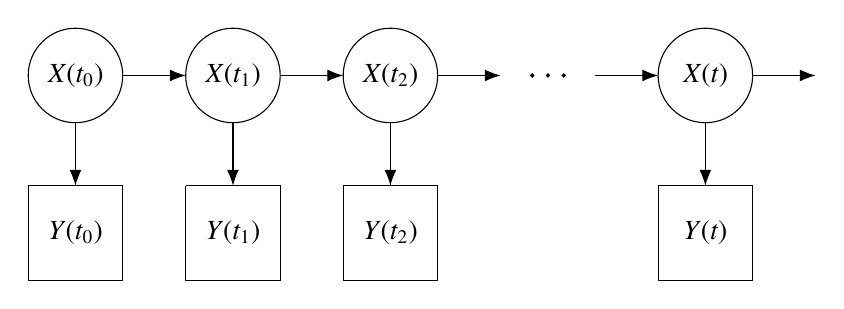
\begin{tikzpicture}
\draw
  (0,0) circle [radius=0.6cm] node {$X(t_0)$}
  (2,0) circle [radius=0.6cm] node {$X(t_1)$}
  (4,0) circle [radius=0.6cm] node {$X(t_2)$}
  (8,0) circle [radius=0.6cm] node {$X(t)$};
\filldraw
  (5.8,0) circle [radius=0.2mm]
  (6,0) circle [radius=0.2mm]
  (6.2,0) circle [radius=0.2mm];
\draw[-{Latex[length=2mm]}] (0.6,0) -- (1.4,0);
\draw[-{Latex[length=2mm]}] (2.6,0) -- (3.4,0);
\draw[-{Latex[length=2mm]}] (4.6,0) -- (5.4,0);
\draw[-{Latex[length=2mm]}] (6.6,0) -- (7.4,0);
\draw[-{Latex[length=2mm]}] (8.6,0) -- (9.4,0);
\draw[-{Latex[length=2mm]}] (0,-0.6) -- (0,-1.4);
\draw[-{Latex[length=2mm]}] (2,-0.6) -- (2,-1.4);
\draw[-{Latex[length=2mm]}] (4,-0.6) -- (4,-1.4);
\draw[-{Latex[length=2mm]}] (8,-0.6) -- (8,-1.4);
\draw (-0.6,-1.4) -- (-0.6,-2.6) -- (0.6,-2.6) -- (0.6,-1.4) -- (-0.6,-1.4) (0,-2) node {$Y(t_0)$};
\draw (1.4,-1.4) -- (1.4,-2.6) -- (2.6,-2.6) -- (2.6,-1.4) -- (1.4,-1.4) (2,-2) node {$Y(t_1)$};
\draw (3.4,-1.4) -- (3.4,-2.6) -- (4.6,-2.6) -- (4.6,-1.4) -- (3.4,-1.4) (4,-2) node {$Y(t_2)$};
\draw (7.4,-1.4) -- (7.4,-2.6) -- (8.6,-2.6) -- (8.6,-1.4) -- (7.4,-1.4) (8,-2) node {$Y(t)$};
\end{tikzpicture}
\vfill

\begin{itemize}
	\item Hipóteses
	\begin{itemize}
		\item Erros de medição são independentes entre si
		\item Todas as variáveis são gaussianas (normais multivariadas)
		\item Relações entre as variáveis são lineares
	\end{itemize}
	\item Modelos não-lineares são muito usados na prática, porém são aproximações
\end{itemize}
\end{frame}

\begin{frame}\frametitle{Modelo matemático}
\begin{itemize}
	\item \pause  Evolução no tempo
	\begin{itemize}
		\item $X(t+ \Delta t) = TX(t) + \mathcal N(0, A)$
	\end{itemize}
	\item Observações
	\begin{itemize}
		\item $Y(t) = PX(t) + \mathcal N(0, B)$
	\end{itemize}
	\item \pause  Exemplo:
	\begin{itemize}
		\item Partícula com posição $s$ e velocidade $v$
		\item Velocidade $v$ muda aleatoriamente (movimento browniano)
		\begin{itemize}
			\item Posição $s$ tem movimento mais suave ($C_1$)
		\end{itemize}
		\item Apenas a posição $s$ é medida
		\item \pause  Modelo resultante:
		\begin{itemize}
			\item $X(t) = \left[\begin{matrix} v(t) \\ s(t) \end{matrix}\right]$, $T = \left[\begin{matrix} 1 & 0 \\ \Delta t & 1 \end{matrix}\right]$, $P = \left[\begin{matrix} 0 & 1 \end{matrix}\right]$
			\item $A = \left[\begin{matrix} \sigma^2 \Delta t & \sigma^2 \Delta t^2/2 \\ \sigma^2 \Delta t^2/2 & \sigma^2 \Delta t^3/3 \end{matrix}\right]$
		\end{itemize}
	\end{itemize}
\end{itemize}
\end{frame}

\begin{frame}\frametitle{Inferência}
\begin{itemize}
	\item Estimativa da distribuição de $X(t)$ é representada por uma média $\mu$ (vetor) e variância $\Sigma$ (matriz)
	\item Na passagem do tempo sem observações, a atualização \textit{a priori} (ou predição) é trivial
	\begin{itemize}
		\item $\text{E}[X(t+\Delta t)] = T\text{E}[X(t)]$
		\item $\text{Var}[X(t+\Delta t)] = T\text{Var}[X(t)]T^T + A$
	\end{itemize}
	\item Ao chegar uma nova observação $Y(t)$, a atualização \textit{a posteriori} é feita pela lei de Bayes assumindo distribuição gaussiana
	\begin{itemize}
		\item $\text{Var}[X(t)|Y(t)]^{-1} = \text{Var}[X(t)]^{-1} + P^TB^{-1}P$
		\item $\text{E}[X(t)|Y(t)] = \text{Var}[X(t)|Y(t)]\left(\text{Var}[X(t)]^{-1}\text{E}[X(t)] + P^TB^{-1}Y(t)\right)$
	\end{itemize}
	\item \pause  Contemple a dualidade entre esses dois tipos de eventos!
	\begin{itemize}
		\item Um (\textit{a priori}) atualiza a variância linearmente
		\item O outro (\textit{a posteriori}) atualiza a inversa linearmente
	\end{itemize}
\end{itemize}
\end{frame}

\begin{frame}\frametitle{Um parêntese}
\begin{itemize}
	\item \pause  Situação I (adição de erro):
	$$X + Y, \text{ } X \Perp Y$$
	$$\text E[X + Y] = \text E[X] + \text E[Y]$$
	$$\text{Var}[X + Y] = \text{Var}[X] + \text{Var}[Y]$$
	\item \pause  Situação II (adição de informação):
	$$X = \mathcal N(z, \Sigma_X), \text{ } Y = \mathcal N(z, \Sigma_Y), \text{ } X \Perp Y$$
	$$\widehat z = \arg\max_z P(X, Y; z)$$
	$$\text{Var}[\widehat z]^{-1} = \Sigma_X^{-1} + \Sigma_Y^{-1} $$
	$$\text{Var}[\widehat z]^{-1} \widehat z = \Sigma_X^{-1}X + \Sigma_Y^{-1}Y $$
\end{itemize}
\end{frame}

\begin{frame}\frametitle{O problema dos atrasos}
\begin{itemize}
	\item \pause  Na prática, observações podem chegar com atraso e fora de ordem
	\begin{itemize}
		\item Atrasos de rede, processamento, etc.
	\end{itemize}
	\item \pause  Questionamentos
	\begin{itemize}
		\item É possível computar eventos de observação fora de ordem?
		\item Se atrasos forem frequentes e substanciais, qual é a forma mais eficiente de manter $(\mu, \Sigma)$ atualizada?
		\item Em caso de um atraso muito longo, é possível atualizar $(\mu, \Sigma)$ sem ter que recalcular tudo? \pause
	\end{itemize}
\end{itemize}
\vfill

\text{ }\text{ }\text{ }\text{ }\text{ }\text{ }
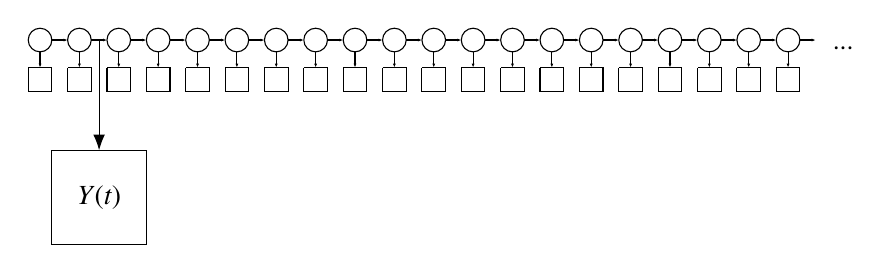
\begin{tikzpicture}
\foreach \x in {0,0.5,1,1.5,2,2.5,3,3.5,4,4.5,5,5.5,6,6.5,7,7.5,8,8.5,9,9.5} {
\begin{scope}[shift={(\x,0)}]
\draw (0,0) circle [radius=0.15cm];
\draw[-{Latex[length=0.5mm]}] (0.15,0) -- (0.35,0);
\draw[-{Latex[length=0.5mm]}] (0,-0.15) -- (0,-0.35);
\draw (-0.15,-0.35) -- (-0.15,-0.65) -- (0.15,-0.65) -- (0.15,-0.35) -- (-0.15,-0.35);
\end{scope}
}
\draw (10.2, -0.1) node {...};
\begin{scope}[shift={(-0.25,0)}]
\draw[-{Latex[length=2mm]}] (1,0) -- (1,-1.4);
\draw (0.4,-1.4) -- (0.4,-2.6) -- (1.6,-2.6) -- (1.6,-1.4) -- (0.4,-1.4) (1,-2) node {$Y(t)$};
\end{scope}
\end{tikzpicture}
\vfill

\end{frame}

\begin{frame}\frametitle{Meta-modelo}
\begin{itemize}
	\item Como modelar uma sequência de eventos de passagem do tempo e observação em uma única operação?
	\begin{itemize}
		\item Passagem do tempo (\textit{a priori}):
		$$\Sigma_\text{new} = T\Sigma_\text{old}T^T + A$$
		$$\mu_\text{new} = T\mu_\text{old}$$
		\item Observação (\textit{a posteriori}):
		$$\Sigma_\text{new}^{-1} = \Sigma_\text{old}^{-1} + P^TB^{-1}P$$
		$$\mu_\text{new} = \Sigma_\text{new}(\Sigma_\text{old}^{-1} + P^TB^{-1}Y)$$
	\end{itemize}
	\item \pause  Vamos pegar emprestado um truque da área de processamento de imagens
\end{itemize}
\end{frame}

\begin{frame}\frametitle{Coordenadas homogêneas}
\begin{itemize}
	\item Adicionar uma dimensão para permitir transformações projetivas (não-lineares)
	$$\left[\begin{matrix} x \\ y \\ 1 \end{matrix}\right] \simeq \left[\begin{matrix} ax \\ ay \\ a \end{matrix}\right] \text{ }\text{ }\text{ } (a \neq 0)$$
\end{itemize}
\vfill

\text{ }\text{ }\text{ }\text{ }\text{ }\text{ }\text{ }\text{ }\text{ }
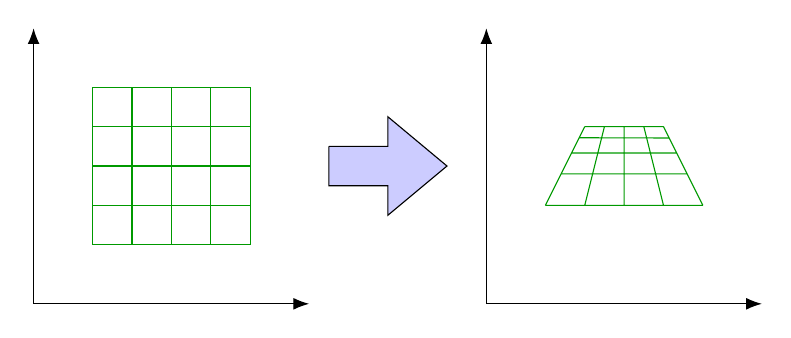
\begin{tikzpicture}
\begin{scope}[shift={(-0.25,-0.25)}]
\draw[-{Latex[length=2mm]}] (0.25,0.25) -- (3.75,0.25);
\draw[-{Latex[length=2mm]}] (0.25,0.25) -- (0.25,3.75);
\draw[green!60!black]
  (1,   1) -- (1,   3)
  (1.5, 1) -- (1.5, 3)
  (2,   1) -- (2,   3)
  (2.5, 1) -- (2.5, 3)
  (3,   1) -- (3,   3)
  (1, 1)   -- (3, 1)
  (1, 1.5) -- (3, 1.5)
  (1, 2)   -- (3, 2)
  (1, 2.5) -- (3, 2.5)
  (1, 3)   -- (3, 3)
;
\end{scope}
\begin{scope}[shift={(-0.75,-1.75)}]
\filldraw[fill=blue!20, draw]
  (4.5, 3.75) --
  (5.25, 3.75) --
  (5.25, 4.125) --
  (6, 3.5) --
  (5.25, 2.875) --
  (5.25, 3.25) --
  (4.5, 3.25) --
  (4.5, 3.75);
\end{scope}
\begin{scope}[shift={(5.5,-0.25)}]
\draw[-{Latex[length=2mm]}] (0.25,0.25) -- (3.75,0.25);
\draw[-{Latex[length=2mm]}] (0.25,0.25) -- (0.25,3.75);
\end{scope}
\begin{scope}[shift={(5.5,-0.75)}]
\draw[green!60!black]
  (1.000,2.000) -- (1.500,3.000)
  (1.500,2.000) -- (1.750,3.000)
  (2.000,2.000) -- (2.000,3.000)
  (2.500,2.000) -- (2.250,3.000)
  (3.000,2.000) -- (2.500,3.000)
  (1.000,2.000) -- (3.000,2.000)
  (1.200,2.400) -- (2.800,2.400)
  (1.333,2.666) -- (2.667,2.666)
  (1.429,2.859) -- (2.571,2.856)
  (1.500,3.000) -- (2.500,3.000)
;
\end{scope}
\end{tikzpicture}
\vfill

\end{frame}

\begin{frame}\frametitle{A ideia}
\begin{itemize}
	\item Decompor $\Sigma = U^{-1}V$ e só atualizar $U$ ou $V$, conforme necessário
	\begin{itemize}
		\item A redundância é intencional
	\end{itemize}
	\item Semelhantemente, decompor $\mu = U^{-1}z$
	\item \pause  Resultado: Os eventos viram multiplicações de matrizes
	\begin{itemize}
		\item \textit{A priori}:
	\end{itemize}
	$$\left[\begin{matrix} U_\text{new} & V_\text{new} & z_\text{new} \end{matrix}\right] = \left[\begin{matrix} U_\text{old} & V_\text{old} & z_\text{old} \end{matrix}\right]\left[\begin{matrix} T^{-1} & T^{-1}A & 0 \\ 0 & T^T & 0 \\ 0 & 0 & 1 \end{matrix}\right]$$
	\begin{itemize}
		\item \textit{A posteriori}:
	\end{itemize}
	$$\left[\begin{matrix} U_\text{new} & V_\text{new} & z_\text{new} \end{matrix}\right] = \left[\begin{matrix} U_\text{old} & V_\text{old} & z_\text{old} \end{matrix}\right]\left[\begin{matrix} I & 0 & 0 \\ P^TB^{-1}P & I & P^TB^{-1}Y \\ 0 & 0 & 1 \end{matrix}\right]$$
\end{itemize}
\end{frame}

\begin{frame}\frametitle{Conclusão}
\begin{itemize}
	\item Uma sequência de atualizações \textit{a priori} e \textit{a posteriori} é um produtório de matrizes
	\item Multiplicação de matrizes não é comutativa (a ordem importa!)
	\item Logo, não é possível manter essas atualizações em $O(1)$

\text{ }\text{ }\text{ }\text{ }\text{ }\text{ }
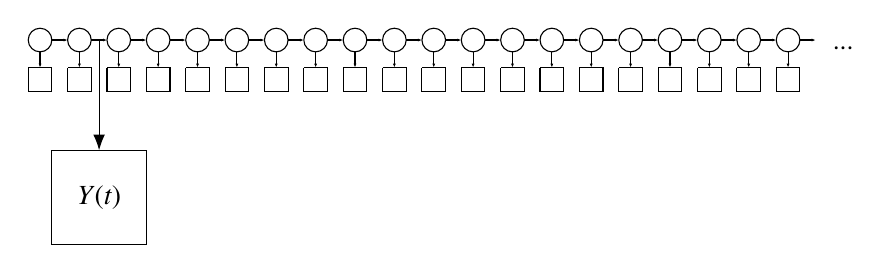
\begin{tikzpicture}
\foreach \x in {0,0.5,1,1.5,2,2.5,3,3.5,4,4.5,5,5.5,6,6.5,7,7.5,8,8.5,9,9.5} {
\begin{scope}[shift={(\x,0)}]
\draw (0,0) circle [radius=0.15cm];
\draw[-{Latex[length=0.5mm]}] (0.15,0) -- (0.35,0);
\draw[-{Latex[length=0.5mm]}] (0,-0.15) -- (0,-0.35);
\draw (-0.15,-0.35) -- (-0.15,-0.65) -- (0.15,-0.65) -- (0.15,-0.35) -- (-0.15,-0.35);
\end{scope}
}
\draw (10.2, -0.1) node {...};
\begin{scope}[shift={(-0.25,0)}]
\draw[-{Latex[length=2mm]}] (1,0) -- (1,-1.4);
\draw (0.4,-1.4) -- (0.4,-2.6) -- (1.6,-2.6) -- (1.6,-1.4) -- (0.4,-1.4) (1,-2) node {$Y(t)$};
\end{scope}
\end{tikzpicture}

	\item \pause  No entanto, é possível atualizar em $O(\log(n))$. Como?
\end{itemize}
\end{frame}

\begin{frame}\frametitle{Conclusão}
Usando uma árvore!
\vfill

\centering
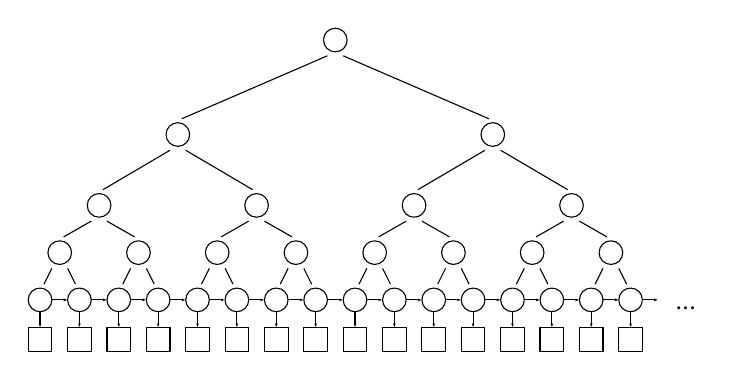
\begin{tikzpicture}
\foreach \x in {0,0.5,1,1.5,2,2.5,3,3.5,4,4.5,5,5.5,6,6.5,7,7.5} {
\begin{scope}[shift={(\x,0)}]
\draw (0,0) circle [radius=0.15cm];
\draw[-{Latex[length=0.5mm]}] (0.15,0) -- (0.35,0);
\draw[-{Latex[length=0.5mm]}] (0,-0.15) -- (0,-0.35);
\draw (-0.15,-0.35) -- (-0.15,-0.65) -- (0.15,-0.65) -- (0.15,-0.35) -- (-0.15,-0.35);
\end{scope}
}
\foreach \x in {0,1,2,3,4,5,6,7} {
\begin{scope}[shift={(\x,0)}]
\draw (0.05, 0.2) -- (0.15,0.4);
\draw (0.45, 0.2) -- (0.35,0.4);
\draw (0.25, 0.6) circle [radius=0.15cm];
\end{scope}
}
\foreach \x in {0,2,4,6} {
\begin{scope}[shift={(\x,0.6)}]
\draw (0.3, 0.2) -- (0.65,0.4);
\draw (1.2, 0.2) -- (0.85,0.4);
\draw (0.75, 0.6) circle [radius=0.15cm];
\end{scope}
}
\foreach \x in {0,4} {
\begin{scope}[shift={(\x,1.2)}]
\draw (0.8, 0.2) -- (1.65,0.7);
\draw (2.7, 0.2) -- (1.85,0.7);
\draw (1.75, 0.9) circle [radius=0.15cm];
\end{scope}
}
\foreach \x in {0} {
\begin{scope}[shift={(\x,2)}]
\draw (1.8, 0.3) -- (3.65,1.1);
\draw (5.7, 0.3) -- (3.85,1.1);
\draw (3.75, 1.3) circle [radius=0.15cm];
\end{scope}
}
\draw (8.2, -0.1) node {...};
\end{tikzpicture}

\begin{itemize}
	\item \pause  Que tipo de árvore?
\end{itemize}
\end{frame}

\begin{frame}\frametitle{Considerações}
\begin{itemize}
	\item \pause  Por que essa ideia não é usada na prática?
	\begin{itemize}
		\item Alto custo de memória
		\item Modelo precisa ser gaussiano e linear
	\end{itemize}
	\item \pause  Ideia não é inédita na literatura
	\begin{itemize}
		\item Representações das atualizações do filtro de Kalman por meio de um ``operador associativo'' já foram propostas
		\item Aplicações incluem paralelização do filtro de Kalman em GPU (ex.: Särkkä e García-Fernández, 2020)
	\end{itemize}
\end{itemize}
\end{frame}

\end{document}
